\chapter{Physical models for charge transport in semiconductor material}
\chaptermark{Physical models}

In this chapter we present the basic physical properties of semiconductor materials according to the quantum mechanics theory \citep{ModernVLSIdevices} and the Drift-Diffusion model \cite{Jackson:ElettroClassica}.

\section{Basic Device Physics}

Because the most used material in the fabrication of VLSI devices technology is silicon, the following description is based on this material choice.

\subsection{Intrinsic semiconductor}
In a silicon crystal each atom has four valence electrons to share with its four neighboring atoms. The valence electrons are shared in a paired configuration called covalent bond.  In a solid semiconductor energy levels of electrons are grouped into bands separated by regions of not allowed energy, the so-called forbidden gaps. The highest energy band completely filled by electrons at 0[K] is called \textit{valence band} ($E_V$), the next band is called \textit{conduction band} ($E_C$).

\begin{figure}[!h]
\centering
\subfloat[][Metal]
{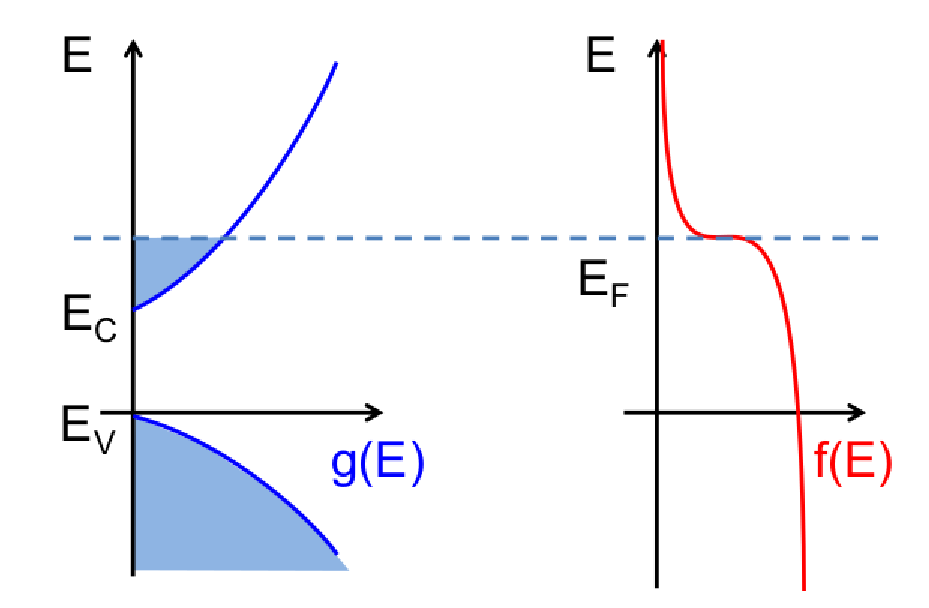
\includegraphics[width=.45\textwidth]{SemiconductorModel/BandeMetalli.eps}}
\psp{5}
\subfloat[][Insulator]
{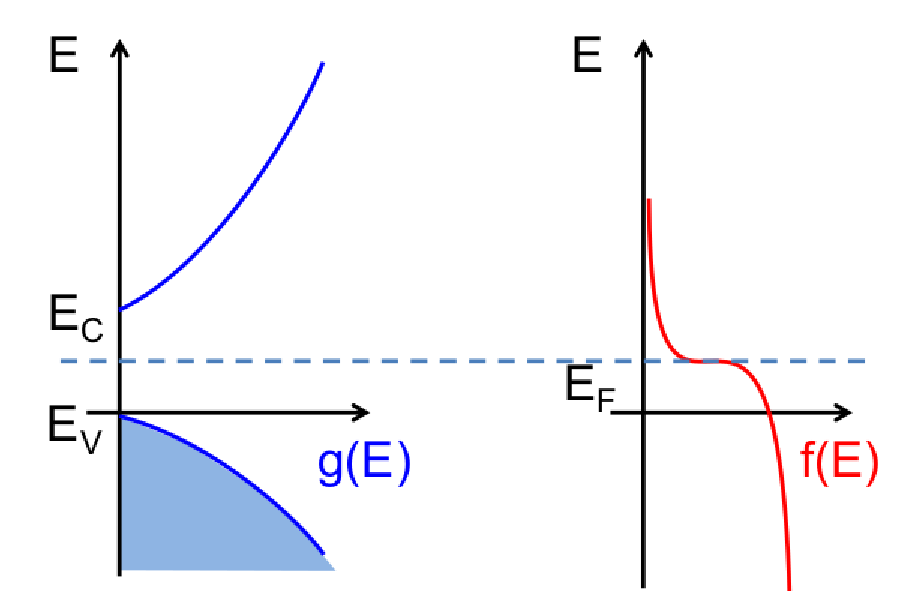
\includegraphics[width=.45\textwidth]{SemiconductorModel/BandeSemiconduttori.eps}}
\caption{Two typical examples of state density occupation (g(E)) and probability distribution (f(E)).  }
\label{fig: density occupation and prob}
\end{figure}

Because in silicon the band gap is 1.11 [eV] \cite{SolidState}, at room temperature a small fraction of the electrons are excited into the conduction band, leaving behind vacancies (called \textit{holes}) in the valence band.
In contrast, an insulator has a much larger forbidden gap making room-temperature conduction virtually impossible, while metals have partially filled conduction bands even at absolute zero temperature, making them excellent conductors at any temperature. 

A suitable formulation of the electron concentration in the conduction band is given by the following integral
\begin{equation}
\label{eq: carrier densiy integral}
n = \int_{E_c}^\infty g(E)f(E) \, dE
\end{equation}
where $g(E)dE$ represents the number of electronic states per unit volume with an energy between $E$ and $E+dE$ in the conduction band and $f(E)$ is the \textit{Fermi-Dirac distribution function}, which gives the probability that an electronic state at energy $E$ is occupied by an electron
\begin{equation}
\label{eq: fermi dirac distribution}
f_D(E) = \dfrac{1}{1+\exp\left(\dfrac{E-E_f}{k_BT}\right)} .
\end{equation}

In \referenzaeq{eq: fermi dirac distribution} $k_B=1.38\times10^{-23}[J/K]$ is Boltzmann's constant, $T$ is the absolute temperature and $E_f$ is the \textit{Fermi level}. 
\figref{fig: density occupation and prob} shows  the state density occupation $g(E)$ and the probability distribution $f(E)$ for a metal and a semiconductor. In order to obtain an analytic formula for the state density occupation $g(E)$, we can consider the well known parabolic approximation of the conduction band \cite{Pierret:SemiFunda}

\begin{equation}
\label{eq: approssimazione banda di conduzione}
E = E_c + \dfrac{\hbar^2}{2m_e^*}\mathrm{k}^2
\end{equation}
where $\hbar=h/2\pi$ and $h=6.63 \times 10^{-34} [J \, s]$ is Planck's constant, $m_e^*$ the electron effective mass, $E_c$ the minimum value of the conduction band and $\mathrm{k}$ the wavenumber. Using this approximation, conduction band density of states can be calculates

\begin{equation}
\label{eq: state density electron}
g(E) = \dfrac{m_e^*\sqrt{2m_e^*(E-E_c)}}{\pi^2\hbar^3}.
\end{equation}

We point that \referenzaeq{eq: carrier densiy integral} is a Fermi integral of order $1/2$ and must be evaluated numerically.
 
\begin{Definizione}
The Fermi level ($E_f$) is the energy at which the probability of occupation of an energy state by an electron is equal to $1/2$.
\end{Definizione}

In most of the cases, when the energy is at least several $k_BT$ above or below the Fermi level (non degenerate semiconductor), equation \referenzaeq{eq: fermi dirac distribution} can be well approximated by the Maxwell-Boltzmann statistics, which reads as follows:

\begin{equation}
\label{eq: maxwell distribution}
f_D(E)\simeq f_{MB}(E) = 
\begin{cases}
\exp\left(-\dfrac{E-E_f}{k_B T}\right) & E\gg E_f \\
1-\exp\left(-\dfrac{E_f-E}{k_BT}\right) & E \ll E_f .
\end{cases}
\end{equation}

The Fermi level plays an essential role for the equilibrium of a system, it is important to keep in mind the following observation.

\begin{Osservazione}
When two systems in contact are in thermal equilibrium with no current flow between them, their Fermi levels must be equal: in other words for a continuous region (of metals or semiconductors in contact), the Fermi level at thermal equilibrium is spatially constant.
\end{Osservazione}

Replacing \referenzaeq{eq: maxwell distribution} and \referenzaeq{eq: state density electron} into \referenzaeq{eq: carrier densiy integral} we obtain

\begin{equation}
n = N_c \exp\left(-\dfrac{E_c-E_f}{k_BT}\right). \label{eq: n density fd}
\end{equation}

Using the similar approach for hole the concentration $p$ in the valence band is

\begin{equation}
p = N_v \exp\left(-\dfrac{E_f-E_v}{k_B T}\right).  \label{eq: p density fd}
\end{equation}

$N_c$ and $N_v$ are the \textit{effective density of states} while $E_v$ is the maximum value of the valence band.
In an intrinsic semiconductor $n=p$ and the \textit{intrinsic Fermi level} $E_i$ can be calculated by \referenzaeq{eq: n density fd} and \referenzaeq{eq: p density fd} as:

\begin{equation}
\label{eq: midgap equilibrium}
E_i=E_f=\dfrac{E_c+E_v}{2} - \dfrac{k_B T}{2}ln\left(\dfrac{N_c}{N_v}\right).
\end{equation}

By replacing \referenzaeq{eq: midgap equilibrium} in \referenzaeq{eq: n density fd} we obtain the the intrinsic carrier concentration $n_i=n=p$

\begin{equation}
\label{eq: ni equilibrium NcNv}
n_i = \sqrt{N_cN_v}exp\left(-\dfrac{E_g}{2k_B T}\right)
\end{equation}
where $E_g=E_c-E_v$ is the semiconductor energy gap.

\begin{Osservazione}
Since the thermal energy, $k_BT$ is much smaller than the usual semiconductor bandgap $E_g$, the intrinsic Fermi level is very close to the midgap.
\end{Osservazione}

Equations \referenzaeq{eq: n density fd} and \referenzaeq{eq: p density fd} can be written in terms of the intrinsic carrier density ($n_i$) and energy ($E_i$) as:

\begin{align}
n & = n_i \exp\left(\dfrac{E_f-E_i}{k_B T}\right) \label{eq: n density mb}\\
p & = n_i \exp\left(\dfrac{E_i-E_f}{k_B T}\right)  \label{eq: p density mb}.
\end{align}

Finally we remark that at thermical equilibrium the \textit{mass action law} holds

\begin{equation}
\label{eq: legge di azione di massa}
np=n_i^2.
\end{equation}


The analysis of the work principles of devices can be effectively done by the band diagram (\figref{fig: band diagram}), which summarizes the information presented above.
\begin{figure}[!h]
\centering
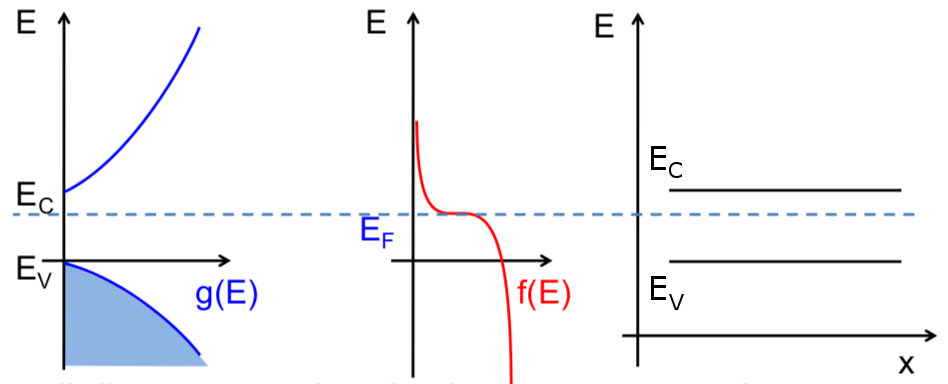
\includegraphics[width=.8\textwidth]{SemiconductorModel/DiagrammaBande.png}
\caption{Construction of the band diagram.}
\label{fig: band diagram}
\end{figure}

\subsection{Extrinsic semiconductor}
At room temperature an intrinsic semiconductor has an extremely low free-carrier concentration, therefore, its resistivity is very high. In order to improve the conductivity of the semiconductor, impurities atoms are added in the material. This introduce additional energy levels in the forbidden gap: the impurities are easily ionized adding either electrons to the conduction band or holes to the valence band, in such a way that the electrical conductivity is dominated by the type and concentration of the impurity atoms.

Two are the types of impurities which are electrically active: those from column V of the Periodic Table such as arsenic or phosphorus, and those from column III such as boron or indium.

The thermal energy at room temperature is sufficient to ionize the impurities and free the extra electron to the conduction band (column V) or accept an electron from valence band (column III). Column V impurities are called \textit{donors}; they become positively charged when ionized. Silicon material doped with column-V impurities or donors is called \textit{n-type} silicon.

Column III impurities are called \textit{acceptors}: they become negatively charged when ionized. Silicon material doped with column-III impurities or acceptors is called \textit{p-type} silicon.

A p-type or an n-type is named as \textit{extrinsic} silicon.
In terms of the energy-band diagram, donors add allowed electron states in the bandgap close to the conduction-band edge, while acceptors add allowed states just above the valence-band edge.

The Fermi level in n-type silicon moves up towards the conduction band while in p-type silicon it moves down towards the valence band. This behaviour is presented in the band diagrams of \figref{fig: Band diagrams of extrinsic silicon}.
The position of the Fermi level depends on both the ionization energy and the concentration of dopants. For the sake of simplicity we consider that at room temperature all impurties are ionized ($N_d = N_d^+$ and $N_a = N_a^-$).  For an n-type material with a donor impurity concentration, $N_d$, the charge neutrality condition requires that
\begin{equation}
\label{eq: equilibrium charge in n-type}
n = N_d^+ + p
\end{equation}
 where $N_d^+$ is the density of ionized donors.  Similarly for a p-type material with acceptor impurity concentration $N_a$ we have
\begin{equation}
\label{eq: equilibrium charge in p-type}
p = N_a^- + n
\end{equation}
 
 Because the magnitude of impurities is in the range of $10^{16}\div 10^{20} [cm^{-3}]$, and intrinsic carrier concentration in the order of $10^{10}[cm^{-3}]$, we can approximate the carrier concentrations as:
  
\begin{equation}
\label{eq: equilibiurm approximation}
\begin{array}{lcl}
n \simeq N_d^+,&\qquad & p \simeq \dfrac{n_i^2}{N_d^+} \psp{8} (n-type)\\ \\
p \simeq N_a^-,& \qquad & n \simeq \dfrac{n_i^2}{N_a^-} \psp{8} (p-type).
\end{array}
\end{equation}

Replacing \referenzaeq{eq: equilibiurm approximation} in  \referenzaeq{eq: n density fd} and \referenzaeq{eq: p density fd} in \referenzaeq{eq: equilibrium charge in n-type} and \referenzaeq{eq: equilibrium charge in p-type} and solving the corresponding algebraic equation, we have:
 
 \begin{align}
 E_c-E_f & = k_B T\ln\left(\dfrac{N_c}{N_d^+}\right)  \label{eq: Ef in n-type}\\
 E_f-E_v & = k_B T\ln\left(\dfrac{N_v}{N_a^-}\right) . \label{eq: Ef in p-type}
 \end{align}

Equation \referenzaeq{eq: Ef in n-type} and \referenzaeq{eq: Ef in p-type} can be written in a more useful form using \referenzaeq{eq: ni equilibrium NcNv} and \referenzaeq{eq: midgap equilibrium} (for $n_i$ and $E_i$):

 \begin{align}
 E_f-E_i & = k_B T\ln\left(\dfrac{N_d^+}{n_i}\right)  \label{eq: Ef in n-type Ei} \\
 E_i-E_f & = k_B T\ln\left(\dfrac{N_a^-}{n_i}\right).  \label{eq: Ef in p-type Ei} 
 \end{align}



\begin{Osservazione}
The distance between the Fermi level and the intrinsic Fermi level is a logarithmic function of doping concentration.
\end{Osservazione}


\begin{figure}[!h]
\centering
\subfloat[][n-type]
{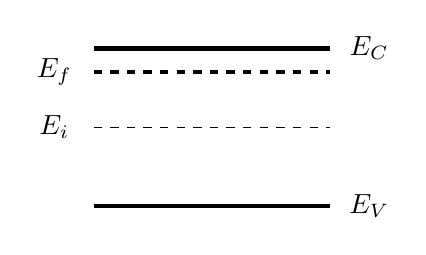
\begin{tikzpicture}
[scale=1.0]
\def\Ecxa{0.0}
\def\Ecya{2}
\def\Ecxb{3}
\def\Ecyb{2}

\def\Evxa{\Ecxa}
\def\Evya{0}
\def\Evxb{\Ecxb}
\def\Evyb{0}

\def\Efxa{\Ecxa}
\def\Efya{1.7}
\def\Efxb{\Ecxb}
\def\Efyb{1.7}

\def\Eixa{\Ecxa}
\def\Eiya{1}
\def\Eixb{\Ecxb}
\def\Eiyb{1}

\node at (\Ecxb+0.5,\Ecyb){$E_C$};
\node at (\Evxb+0.5,\Evyb){$E_V$};
\node at (\Efxa-0.5,\Efya){$E_f$};
\node at (\Eixa-0.5,\Eiya){$E_i$};

\draw[ultra thick](\Ecxa,\Ecya)--(\Ecxb,\Ecyb);
\draw[ultra thick](\Evxa,\Evya)--(\Evxb,\Evyb);
\draw[ultra thick,dashed](\Efxa,\Efya)--(\Efxb,\Efyb);
\draw[dashed](\Eixa,\Eiya)--(\Eixb,\Eiyb);
\end{tikzpicture}}
\psp{20}
\subfloat[][p-type]
{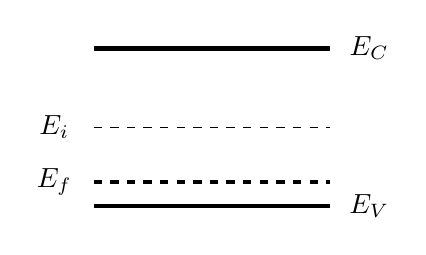
\begin{tikzpicture}
[scale=1.0]
\def\Ecxa{0.0}
\def\Ecya{2}
\def\Ecxb{3}
\def\Ecyb{2}

\def\Evxa{\Ecxa}
\def\Evya{0}
\def\Evxb{\Ecxb}
\def\Evyb{0}

\def\Efxa{\Ecxa}
\def\Efya{0.3}
\def\Efxb{\Ecxb}
\def\Efyb{0.3}

\def\Eixa{\Ecxa}
\def\Eiya{1}
\def\Eixb{\Ecxb}
\def\Eiyb{1}

\node at (\Ecxb+0.5,\Ecyb){$E_C$};
\node at (\Evxb+0.5,\Evyb){$E_V$};
\node at (\Efxa-0.5,\Efya){$E_f$};
\node at (\Eixa-0.5,\Eiya){$E_i$};

\draw[ultra thick](\Ecxa,\Ecya)--(\Ecxb,\Ecyb);
\draw[ultra thick](\Evxa,\Evya)--(\Evxb,\Evyb);
\draw[ultra thick,dashed](\Efxa,\Efya)--(\Efxb,\Efyb);
\draw[dashed](\Eixa,\Eiya)--(\Eixb,\Eiyb);
\end{tikzpicture}}
\caption{Band diagrams of extrinsic silicon for \referenzaeq{eq: Ef in n-type Ei} and \referenzaeq{eq: Ef in p-type Ei}.}
\label{fig: Band diagrams of extrinsic silicon}
\end{figure}

\subsection{Carrier densities at nonequilibrium condition}

In VLSI device a nonequilibrium condition is often possible: the densities of one or both types of carriers depart from their equilibrium as given by \referenzaeq{eq: n density mb} and \referenzaeq{eq: p density mb}.
In particular, the minority carrier concentration can be easily overwhelmed by the injection from neighboring regions. Under these circumstances, while electrons and holes are in local equilibrium with themselves, they are not in equilibrium with each other. In order to extend the relationship between Fermi level and densities discussed above, we can introduce different Fermi levels for electrons and holes. They are called \textit{quasi Fermi levels} defined as:

\begin{align}
E_{fn} = E_i + k_B T \ln\left( \dfrac{n}{n_i} \right) \label{eq: quasi fermi level electron} \\
E_{fp} = E_i - k_B T \ln\left( \dfrac{p}{n_i} \right). \label{eq: quasi fermi level hole}
\end{align}


Considering the well known relation between electrostatic potential and energy $\varphi = -E/q$, \referenzaeq{eq: quasi fermi level electron} and \referenzaeq{eq: quasi fermi level hole} can be written as:

\begin{align}
n & = n_i \exp\left(\dfrac{\varphi_{i}-\varphi_n}{k_BT/q}\right) \label{eq: non eq n density mb}\\
p & = n_i \exp\left(\dfrac{\varphi_p-\varphi_{i}}{k_BT/q}\right)  \label{eq: non eq p density mb}
\end{align}
where $\varphi_n$ and $\varphi_p$ are the quasi Fermi potential levels and $\varphi_i$ is the midgap potential level, while $q=1.602e^{-19}[C]$ is the elementary charge. 

\begin{Osservazione}
In non equilibrium condition quasi Fermi levels have the same physical meaning in terms of the state occupancy as the Fermi level, therefore the electron (hole) density in the conduction band can be calculated using $E_{fn}$ ($E_{fp}$).
\end{Osservazione}

\subsection{Carrier transport in a semiconductor}
\label{sec: carrier transport}

Carrier transport or current flow is driven by two different mechanisms:
\begin{itemize}
\item the \textbf{drift}, which is caused by the presence of an electric field;
\item the \textbf{diffusion}, which is caused by a spatial gradient of electron or hole concentration.
\end{itemize}

\subsubsection{Drift current - Ohm's law}

When an electric field is applied to a device, the free carriers are accelerated and acquire a drift velocity superimposed upon their random thermal motion.

\begin{Osservazione}
The drift velocity of holes ($h$) is in the direction of the applied field, and the drift velocity of electrons ($e$) is opposite to the field.
\end{Osservazione}

The velocity of the carriers does not increase indefinitely under field acceleration, since they are scattered frequently and lose their acquired momentum after each collision.
During their motion throughout the lattice structure, carriers travel at an average speed defined by:
\begin{equation}
\label{eq: velocities}
\vect{v}_d^e = - \dfrac{q\vect{E}\tau_e}{m_e^*} \, , \psp{20} 
\vect{v}_d^h = + \dfrac{q\vect{E}\tau_h}{m_h^*}
\end{equation}
where $\vect{E}$ is the electric field, $\tau_e$, $\tau_h$ the average times between two consecutive scattering events and $m_e^*$, $m_h^*$ the effective masses of electron and hole respectively.
The coefficient $q\tau_e / m_e$ ($q\tau_p / m_p$) characterizes how quickly a carrier move through the lattice and is known as carrier mobility $[cm^2V^{-1}s^{-1}]$.
In general, to include different scattering mechanisms \textit{Matthiessen's rule} is used to calculate the resulting mobility
\begin{equation}
\dfrac{1}{\mu} = \dfrac{1}{\mu_L} + \dfrac{1}{\mu_I} + \cdots
\end{equation}
where $\mu_L$ and $\mu_I$ correspond to the lattice and impurity scattering (for a more detailed description of mobility models see \cite{ModernVLSIdevices}). 

Therefore the drift electron (hole) current density, reads as follows:

\begin{align}
\vect{J}_n =& -qn\vect{v}_d^n = qn\mu_n\vect{E}   = \sigma_n\vect{E} \label{eq: drift electron} \\ 
\vect{J}_p =& +qp\vect{v}_d^p = qp\mu_p\vect{E} = \sigma_p\vect{E}. \label{eq: drift hole}
\end{align}

The scalar coefficient $qn\mu_n(qp\mu_p)$ is called electron (hole) conductivity $\sigma_n(\sigma_p)$. 

Relations \referenzaeq{eq: drift electron} and \referenzaeq{eq: drift hole} express the well known \textit{Ohm' law} stating that the current density is directly proportional to the applied electric field.


\subsubsection{Diffusion current - Fick's law}

In semiconductor devices it is very common to have different profiles of dopant in order to allow specific electrical behaviors. This implies a non uniform concentration of carriers which also diffuse as a result of a gradient concentration. This leads to an additional current contribution accordingly to the classical \textit{Fick's law}:
\begin{align}
\vect{J}_n = -D_n(-q\nabla n) \label{eq: diff electron}\\
\vect{J}_p = -D_p(+q\nabla p) . \label{eq: diff hole}
\end{align}

The constants $D_n$ and $D_p$ are called electron and hole diffusion coefficients and have units of $[cm^2s^{-1}]$. Drift and diffusion are closely associated with the random thermal motion of carriers and their collisions with the silicon lattice in thermal equilibrium. The \textit{Einstein relation} \referenzaeq{eq: einstein relation} expresses the relation between diffusivity and mobility

\begin{equation}
\label{eq: einstein relation}
D_n = \dfrac{k_BT}{q}\mu_n, \qquad D_p = \dfrac{k_BT}{q}\mu_p.
\end{equation}

\subsubsection{Drift-Diffusion transport equations}
\label{subsub:driftdiffusion transport}

By considering \referenzaeq{eq: drift electron}, \referenzaeq{eq: drift hole}, \referenzaeq{eq: diff electron} and \referenzaeq{eq: diff hole}, the electron and hole current densities become \cite{selberherr:SimSem} is:

\begin{align}
\vect{J}_n &= qn\mu_n\vect{E} + qD_n\nabla n  \label{eq: drift diff electron}\\ 
\vect{J}_p &= qp\mu_p\vect{E} - qD_p \nabla p. \label{eq: drift diff hole}
\end{align}
The total conduction current density is

\begin{equation*}
\vect{J}=\vect{J}_n+\vect{J}_p.
\end{equation*}


Equations \referenzaeq{eq: drift diff electron} and \referenzaeq{eq: drift diff hole} are called constitutive laws and they can be written in two other ways highlighting different physical explanations of the same phenomenon. These interpreations give also different starting points for the mathematical formulation and solution of the Drift-Diffusion model.

Considering that the electric field is related to the scalar potential through the quasi-static approximation
\begin{equation}
\label{eq: relazione pot electric}
\vect{E}  = -\nabla \varphi ,
\end{equation}
using \referenzaeq{eq: einstein relation} the current densities can be written as:

\begin{align}
\vect{J}_n &= -qn\mu_n\left(\nabla \varphi - \dfrac{k_BT}{qn}\nabla n \right) \label{eq: Jn DD} \\ 
\vect{J}_p &= -qp\mu_p\left(\nabla \varphi+ \dfrac{k_BT}{qp} \nabla p \right). \label{eq: Jp DD}
\end{align}

Considering equations \referenzaeq{eq: non eq n density mb} and \referenzaeq{eq: non eq p density mb} the above are equal to:

\begin{align}
\vect{J}_n = -qn\mu_n\nabla \varphi_n \label{eq: Jn qf}\\
\vect{J}_p = -qp\mu_p\nabla \varphi_p \label{eq: Jp qf}.
\end{align}

With these equations we underly an important aspect which occurs in a semiconductor:
\begin{Osservazione}
The current density is proportional to the gradient of the quasi Fermi potential.
\end{Osservazione}

The third way to represent the current density is based on \textit{Slotboom variables} which are particularly suited for the mathematical analysis of the semiconductor equations:

\begin{align}
u_n &= n_i\exp\left(-\dfrac{\varphi_n}{V_{th}} \right) \label{eq: un slotboom} \\
u_p &= n_i\exp\left(\dfrac{\varphi_p}{V_{th}} \right) \label{eq: up slotboom} 
\end{align}
where $V_{th}=k_BT/q$. Put these equations into \referenzaeq{eq: drift diff electron} and \referenzaeq{eq: drift diff hole} we obtain:

\begin{align}
\vect{J}_n &= qD_n \exp\left(\dfrac{\varphi}{V_{th}}\right) \nabla u_n \label{eq: Jn slotboom} \\
\vect{J}_p &= -qD_p \exp\left(-\dfrac{\varphi}{V_{th}}\right)  \nabla u_p .\label{eq: Jp slotboom}
\end{align}

\begin{Osservazione}
The drift-diffusion current density in a semiconductor is a purely diffusive flux of a new kind of carrier with a properly modified diffusion coefficient. 
\end{Osservazione}


\section{Drift Diffusion Model for semiconductors}
\label{section: dd model for semi}

To the study of integrated devices \textit{Drift Diffusion model} (DD) is becomed the most widely used mathematical approach in particular in industrial simulation. In this section we show how the DD model can be obtained.

\subsection{Drift Diffusion formulation}
 The system of Maxwell equations describes the propagation of electromagnetic signal in a medium \cite{Jackson:ElettroClassica}:

\begin{align}
\nabla \times \vect{H} & =  \vect{J} + \dfrac{\partial \vect{D}}{\partial t} \label{eq: magnetic equation} \\ 
\nabla \times \vect{E} & =  - \dfrac{\partial \vect{B}}{\partial t} \label{eq: ampere law}\\ 
\nabla \cdot \vect{D} & =  \rho \label{eq: gauss law}\\ 
\nabla \cdot \vect{B} &  =  0 \label{eq: no magetic charge law}
\end{align}
with the following set of constitutive laws that characterize the electromagnetic properties of the medium:

\begin{equation}
\begin{array}{rcl}
\vect{D} & = & \epsilon \vect{E} \\
\vect{B} & = & \mu_m \vect{H} \label{eq: magnetic costitutive}
\end{array}
\end{equation}
where $\epsilon$ is the material dielectric permettivity $[F cm^{-1}]$ and $\mu_m$ is the magnetic permeability $[H cm^{-1}]$. Since $\nabla \cdot (\nabla \times \vect{A})=0$ for any vector $\vect{A}$, \referenzaeq{eq: no magetic charge law} is satisfied by introducing a vector potential $\vect{A}$ such that $\vect{B}= \nabla \cdot \vect{A}$. We replace it in \referenzaeq{eq: ampere law} to obtain

\begin{equation}
\nabla \times \left( \vect{E} + \dfrac{\partial \vect{A}}{\partial t} \right) = 0.
\end{equation}

From this we can state that there exists a scalar potential $\varphi$ such that

\begin{equation}
\label{eq: potenziale scalare}
\vect{E} + \dfrac{\partial \vect{A}}{\partial t} = -\nabla \varphi.
\end{equation}


 Applying the divergence operator and using \referenzaeq{eq: relazione pot electric}, \referenzaeq{eq: magnetic costitutive} and \referenzaeq{eq: gauss law}, relation \referenzaeq{eq: potenziale scalare} becomes

\begin{equation}
\rho + \dfrac{\partial \vect{A}}{\partial t}  = -\nabla \cdot (\epsilon \nabla \varphi).
\end{equation}

We now assume that $\dfrac{\partial \vect{A}}{\partial t} = 0$ (quasi static approximation) and we have the \textit{Poisson Equation}

\begin{equation}
\label{eq: Poisson equation}
\nabla \cdot (\epsilon \nabla \varphi) = \rho.
\end{equation} 
	
Applying the divergence operator to \referenzaeq{eq: magnetic equation} and considering \referenzaeq{eq: Poisson equation} we get the \textit{Continuity Equation}

\begin{equation}
\label{eq: continuity equation total}
\dfrac{\partial \rho}{\partial t} + \nabla \cdot \vect{J}  =  0. \end{equation} 


To close system  given by \referenzaeq{eq: Poisson equation} and \referenzaeq{eq: continuity equation total}, we need to specify the mathematical form of the electric charge density ($\rho$) and the electric conduction current density ($\vect{J}$).
Considering \referenzaeq{eq: equilibiurm approximation} $\rho$ can be expressed as


\begin{equation}
\label{eq: charge balance}
\rho = \underbrace{q(p-n)}_{\rho_{free}} +\underbrace{q(N_D-N_A)}_{\rho_{fixed}}
\end{equation}

in which we can distinguish the two following contributions:

\begin{itemize}
\item free charge ($\rho_{free}$) (free electron and holes carriers),
\item fixed charge ($\rho_{fixed}$) (ionoized dopant impurities).
\end{itemize} 


 Notice that we assume $N_D^+$ and $N_A^-$ to be time invariant ($\partial N_D^+ / \partial t=\partial N_A^- / \partial t = 0$).

 Splitting the continuity equation \referenzaeq{eq: continuity equation total} into two distinct equations (for holes and electrons) Drift Diffusion (DD) model formulation reads as follows:
  
\begin{equation}
\label{eq: full problem}
\left\{
\begin{array}{rcl}
\nabla \cdot (-\epsilon \nabla \varphi) & = & q(p-n+N_D^+-N_A^-)\\ \\
-q\dfrac{\partial n}{\partial t} + \nabla \cdot ( - q\mu_n n \nabla \varphi + qD_n \nabla n )& = & qR\\ \\
q\dfrac{\partial p}{\partial t} + \nabla \cdot (- q\mu_p p \nabla \varphi - qD_p \nabla p )& = & -qR 
\end{array}
\right.
\end{equation}

where the arbitrarily introduced function $R=R(\vect{x},t)$ can be considered as the net rate of generation and recombination.
The system is an incompletely parbolic initial value/boundary problem in three scalar unknown dependent variables $\varphi(\vect{x},t)$, $n(\vect{x},t)$ and $p(\vect{x},t)$: the presence of the drift terms ($n\nabla \varphi$ and $p \nabla 	\varphi$) makes \referenzaeq{eq: full problem} a nonlinear coupled system of PDE's. 

From Maxwell equations we are able to guarantee only that $\vect{J}$ is a solenoidal field.
The stationary form can be easily deduced from \referenzaeq{eq: full problem} by neglecting the temporal derivatives.





\subsection{Generation and Recombination phenomenon}
\label{subsection: RG}

The modelling of $R(\vect{x},t)$ is fundamental for device simulation due to its role in determining the current-voltage characteristic.
 
It is important to keep in mind that electrons and holes are in continuos fluctuation due to their thermal energy, the macroscopic result is that the net recombination rate at equilibrium  is identically zero. Our interest is to analyze the deviations from this condition. 

While generation events are usually due to thermal agitation or an external input source, the recombination events happen in order to neutralize an excess of charge.

The phenomenological model for the net recombination rate $R$ is often given in the following

\begin{equation}
\label{eq: generic RG}
R(n,p) = (pn-n_i^2)F(n,p)
\end{equation}

where $F$ is a function accounting for specific recombination/generation (R/G) events.
In the following we present the classical theory that includes three specific kind of contributions. 

\subsubsection{Shockley-Read-Hall recombination (SRH)}

Electron and hole generation and recombination can take place directly between the valence band and the conduction band, or mediated via trap centers in the energy gap. Shockley-Read-Hall phenomena is a two-particle process which matematically expresses the probability that:
\begin{itemize}
\item an electron in the conduction band neutralizes a hole at the valence band through the mediation of an unoccupied trapping level located at the energy gap ($R_{SRH}$),
\item an electron is emitted from the valence band to the conduction band, through the mediation of an unoccupied trapping level located at the energy gap ($G_{SRH}$).
\end{itemize}

The modeling function $F$ is given by

\begin{equation}
F_{SRH}(n,p) = \dfrac{1}{\tau_n\left(p+n_i \cosh\left(\dfrac{E_T}{k_BT} \right) \right)+\tau_p\left(n+n_i \cosh\left(\dfrac{E_T}{k_BT}\right) \right)}
\end{equation}
where $E_T$ is the energy level of the traps, $\tau_n$ and $\tau_p$ are called \textit{carrier lifetimes} and are physically defined as the reciprocals of the capture rates. The typical order of magnitude of the lifetimes lies in the range of $10^{-3}\mu s\div 1 \mu s$ (see  \cite{VanOver:SRH} and \cite{Goebel:SRH}). 

\begin{table}[!h]
\centering
\begin{tabular}{cccc}
\toprule
Parameter & Unit & Electrons & Holes \\
\midrule
$\tau$ & s & $1.0\times 10^{-5}$ & $3.0 \times 10^{-6}$\\
$E_T$ & eV & 0.0 & 0.0\\
\bottomrule
\end{tabular}
\caption{Parameters in the Shockley-Read-Hall generation/recombination model.}
\end{table}

\subsubsection{Auger recombination (AU)}

Auger R/G is a three-particle process and takes place directly between the valence band and the conduction band. We distinguish four cases which depend on the type of carriers involved:

\begin{itemize}[leftmargin=1.5cm]
\item[$R_{AU}^{2n,1p}$] a high-energy electron in the conduction band moves to the valence band where it neutralizes a hole, transmitting the excess energy to another electron in the conduction band;
\item[$G_{AU}^{2n,1p}$] an electron in the valence band moves to the conduction band by taking the energy from a high energy electron in the conduction band and leaves a hole in the valence band;
\item[$R_{AU}^{2p,1n}$] an electron in the conduction band moves to the valence band where it neutralizes a hole, transmitting the excess energy to another hole in the valence band;
\item[$G_{AU}^{2p,1n}$] an electron in the valence band moves to the conduction band by taking the energy from a high energy hole in the valence band and leaves a hole in the valence band.
\end{itemize}

The modeling function $F$ is

\begin{equation}
F_{AU}(n,p) = C_nn+C_pp
\end{equation}
where the quantities $C_n$ and $C_p$ are the so called  Auger capture coefficients tipically in the order of magnitude of $10^{-25}[cm^6s^{-1}]$ \cite{Lochmann}.
Note that Auger R/G is relevant only when both carrier densities are high.

\begin{table}[!h]
\centering
\begin{tabular}{ccc}
\toprule
Parameter & Unit & Magnitude \\
\midrule
$C_n$ & $cm^6s^{-1}$ & $2.9 \times 10^{-31}$ \\
$C_p$ & $cm^6s^{-1}$ & $1.028 \times 10^{-31}$ \\
\bottomrule
\end{tabular}
\caption{Parameters in Auger generation/recombination model.}
\end{table}

\subsubsection{Impact ionization (II)}
\label{sec: ImpactIonization}

The impact ionization mechanism is a three-particle phenomena where carrier generation is triggered by the presence of a high electric field: due to this field an electron could gain enough energy to excite an electron-hole pair out of a silicon lattice bond. Then the process can be repeated until an avalanche of generated carriers is produced within the region: this process can not be described  by a relation of the form \referenzaeq{eq: generic RG}. 

Among the different formulations for the impact ionization generation we choose the van Overstraeten - de Man model \cite{VanOverII}, based on the Chynoweth law \cite{Cynoweth}:

\begin{equation}
G_{II}(n,p)= \alpha_n n |\vect{v}_n| + \alpha_p p |\vect{v}_p|
\end{equation}

with:

\begin{equation}
\alpha(E_{ava}) = \gamma a \exp\left(-\dfrac{\gamma b}{E_{ava}} \right)
\end{equation} 
\begin{equation}
\gamma = \dfrac{\tanh\left(\dfrac{\hbar \omega_{op}}{2k_BT_0} \right) }{\tanh\left(\dfrac{\hbar \omega_{op}}{2k_BT} \right)}
\end{equation}
where $\hbar \omega_{op}$ is the phonon energy, $b$ the critical electric field and $\gamma$ the temperature dependence of the phonon gas against which carriers are accelerated. Two sets of coefficients $a$ and $b$ are used for high and low ranges of electric field. The values $a_{low}$, $b_{low}$ are used in the low field range up to $E_{0}$ and the values $a_{high}$, $b_{high}$ apply in the high field above $E_0$. $E_{ava}$ is the driving force that can be computed as:
\begin{itemize}
\item the component of the electrostatic field in the direction of current flow
\begin{equation}
E_{ava}^{n,p} = \dfrac{\vect{E}\cdot\vect{J}_{n,p}}{||\vect{J}_{n,p}||}
\end{equation}
\item the module of the quasi fermi gradient
\begin{equation}
E_{ava}^{n,p} = |\nabla \varphi_{n,p}|.
\end{equation}
\end{itemize}

\begin{table}[!h]
\centering
\begin{tabular}{ccccc}
\toprule
Parameter & Unit & Electrons & Holes  & Valid range of electric field\\
\midrule
$E_0$ & $V \, cm^{-1}$ & $4.0 \times 10^{5}$ & $4.0 \times 10^{5}$ & \\
$a_{high}$ & $cm^{-1}$ & $7.03 \times 10^{5}$ & $6.71 \times 10^{5}$ & $E_0$ to $6.0 \times 10^{5}$\\
$a_{low}$ & $cm^{-1}$ & $7.03 \times 10^{5}$ & $1.582 \times 10^{6}$ & $1.75 \times 10^{5}$ to $E_0$\\
$b_{high}$ & $V \, cm^{-1}$ & $1.231 \times 10^{6}$ & $1.693 \times 10^{6}$ & $E_0$ to $6.0 \times 10^{5}$\\
$b_{low}$ & $V \, cm^{-1}$ & $1.231 \times 10^{6}$ & $2.036 \times 10^{6}$ &$1.75 \times 10^{5}$ to $E_0$\\
$\hbar\omega_{op}$ & eV & 0.063 & 0.063\\
\bottomrule
\end{tabular}
\caption{Parameters in van Overstraeten-de Man model.}
\end{table}



\subsection{Mobility models}

In this section we illustrate the most common phenomenological models for carrier mobilities. The main physical phenomena underlying a mobility reduction with respect to the bulk are:

\begin{itemize}
\item interaction with the silicon atoms (due to thermal vibrations);
\item interaction with ionized dopant impurities in the crystal.
\end{itemize}

\subsubsection{Scattering with lattice}

Carrier mobility is a decreasing function of temperature, as we expect collisions become more and more frequent as T gets higher (see \cite{Lombardi:MobConst}). This can be represented by

\begin{equation}
\label{eq: mobility thermal}
\mu_\nu^L = \mu_\nu^0\left( \dfrac{T}{T_0}\right)^{-\beta_\nu} \psp{15} \nu = n,p
\end{equation}

where $\mu_\nu^0$ is the low-field mobility, $\beta_\nu$ positive numbers and $T_0$ is a reference temperature $T_0=300[K]$.

\begin{table}[!h]
\centering
\begin{tabular}{cccc}
\toprule
Parameter & Unit & Electrons & Holes \\
\midrule
$\mu^0$ & $cm^2V^{-1}s^{-1}$ & 1417.0 & 470.5\\
$\beta$ & 1 & 2.5 & 2.2\\
\bottomrule
\end{tabular}
\caption{Parameters for mobility models including scattering from lattice thermal vibrations.}
\end{table}

\subsubsection{Scattering from ionized impurities}
\label{sec: Masetti model}

Dopant ionized impurities induce local perturbations of the periodic silicon lattice, they strongly influence the carrier motion through electrostatic interaction, reducing the mobility. To take into account this physical effect the following model has been proposed in \cite{Masetti:MobDop}


\begin{equation}
\label{eq: mobility impurities}
\mu = \mu_{min1}\exp\left( 	- \dfrac{P_c}{N_{tot}}\right)
 + \dfrac{\mu^L-\mu_{min2}}{1 + \left( \dfrac{N_{tot}}{C_r} \right)^{\alpha} } 
 - \dfrac{\mu_1}{1 + \left( \dfrac{C_s}{N_{tot}} \right)^{\beta} } 
\end{equation}
where $N_{tot} = N_D^+ + N_A^-$, $\mu_\nu^L$ is given by \referenzaeq{eq: mobility thermal}, $\mu_{min1}$ and $\mu_{min2}$  are the minimum values of $\mu$; $P_c$, $C_r$ and $C_s$ are reference doping values.


\begin{table}[!h]
\centering
\begin{tabular}{cccc}
\toprule
Parameter & Unit & Electrons & Holes \\
\midrule
$\mu_{min1}$ & $cm^2V^{-1}s^{-1}$ & 52.2 & 44.9\\
$\mu_{min2}$ & $cm^2V^{-1}s^{-1}$ & 52.2 & 0\\
$\mu_1$ & $cm^2V^{-1}s^{-1}$ & 43.4 & 29.0 \\
$P_c$ & $cm^{-3}$ & 0 & $9.23\times 10^{16}$\\
$C_r$ & $cm^{-3}$ &  $9.68\times 10^{16}$ & $2.23\times 10^{17}$ \\
$C_s$ & $cm^{-3}$ & $3.43\times 10^{20}$ & $6.10\times 10^{20}$\\
$\alpha$& 1 & 0.680 & 0.719  \\
$\beta$& 1 & 2.0 & 2.0 \\
\bottomrule
\end{tabular}
\caption{Parameters for models including scattering from ionized dopant impurities.}
\end{table}


\subsubsection{Veclocity saturation at high electric field}

Under the assumption of low electric field, mobilities are reasonably constant and the carrier drift velocity is proportional to the electric field. As the applied field strength increases, the above assumption predicts an unbounded carrier velocity as $|\vect{E}| \rightarrow \infty$. This outcome is physical incorrect, indeed at high fields, carriers lose their energy by optical-phonon emission \cite{ModernVLSIdevices}. We can take this into account by considering that

\begin{equation}
\label{eq: velocity saturation}
\lim_{|\vec{E}| \to \infty} \mu |\vect{E}| = v_{sat}.
\end{equation} 

A common adopted formula is the \textit{Canali model} \cite{Canali:Vsat}

\begin{equation}
\label{eq: mobility canali}
\mu = \dfrac{\mu_{L}}{\left[ 1 + \left( \dfrac{\mu_{L}|\vect{E}|}{v_{sat}} \right)^{\beta}   \right]^{1/\beta}} 
\end{equation}

where $\mu_L$ is \referenzaeq{eq: mobility thermal} while $v_{sat}$ and $\beta$ are given by

\begin{equation}
\label{eq: mobility canali beta}
v_{sat} = v_0exp\left( 	\dfrac{300}{T} \right)^{v_{exp}} 
\psp{15}
\beta= \beta_0 \left( \dfrac{T}{300} \right)^{\beta_{exp}}.
\end{equation}

where $v_0$ and $\beta_{exp}$ are fitting parameters.

\begin{table}[!h]
\centering
\begin{tabular}{cccc}
\toprule
Parameter & Unit & Electrons & Holes \\
\midrule
$v_0$ & $cm\,s^{-1}$ & $1.07\times 10^{7}$ & $8.37\times 10^{6}$\\
$v_{exp}$ & 1 & 0.87 & 0.52\\
$\beta_0$ & 1 & 1.109 & 1.213 \\
$\beta_{exp}$ & 1 & 0.66 & 0.17\\
\bottomrule
\end{tabular}
\caption{Parameters for mobility models including scattering from velocity saturation.}
\end{table}

